\documentclass[a4paper]{article}

\usepackage[english]{babel}
\usepackage[utf8]{inputenc}
\usepackage{amsmath}
\usepackage{graphicx}
\usepackage[colorinlistoftodos]{todonotes}
\usepackage[numbers]{natbib}

%Import the natbib package and sets a bibliography  and citation styles
\usepackage{natbib}
\bibliographystyle{abbrvnat}
\setcitestyle{authoryear,open={(},close={)}}

\title{Using planktonic foraminifera assemblages to assess biases in museum historical collections}

\author{Marina C. Rillo, Michal Kučera, Thomas H. G. Ezard, \\ Andy Purvis \& C. Giles Miller}

\date{\today}

\begin{document}
\maketitle

%\begin{abstract}
%Enter a short summary here. What topic do you want to investigate and why? What experiment did you perform? What were your main results and conclusion?
%\end{abstract}

%----------------------------------------------------------------------------------------

\section{Introduction}
\label{sec:intro}

\paragraph{(General intro: importance of museum collections and specially historical collections)}
Although historical samples are an important resource of recent past data \citep{lister2011natural}, they often hold imprecise information about the sampling method or the method itself was inaccurate at the time. Here, we assessed potential sampling biased in two historical collections held by the Natural History Museum in London (NHMUK). We used planktonic foraminifera assemblages to study these biases.

The first historical collection studied is the Ocean-Bottom Deposits (OBD) Collection held by the NHMUK. This collection consists of about 40,000 samples from all the world's oceans and is the most comprehensive British collection of seabed samples and cores.
The OBD samples collected during many of the famous marine expeditions on the 19th and 20th centuries, including the important HMS Challenger expedition which took place 150 years ago (1872-76) and sailed around the globe.
The OBD collection is thus invaluable for studies of the ocean and ocean floor, including research looking at global change, including ocean acidification and marine pollution over the last century. 
The sampling of the sea floor before the 1970s (?) was inaccurate, usually the exact depth below the sea floor sampled was not measured and techniques such as dredging, sounding and collecting sediments from the anchor were applied. 
Sediment age estimation is thus imprecise and could include mixed sediments of the Holocene (last 11,700 years, \citealt{walker2008global}) and the Last Glacial Maximum (LGM, 21,000 years ago, \citealt{margo2009lgm}).
This potential bias leads to a under-use of historical oceanographic collections such as the OBD Collection.
% The sediment/sample depths (i.e. depth below sea floor) were reported in the expeditions from the 20th century. For expeditions from the 19th century, I retrieved the sea floor sampling method from the NHMUK archive (Table \ref{Table2_SampleVessels}, column \emph{Dbsf}).

Another historical collection held by the NHMUK is the Henry Buckley Planktonic Foraminifera Collection. Henry Buckley sampled sediments from the NHMUK OBD Collection to mount a specimens slides collection of modern planktonic foraminifera species (Rillo et al 2016). Good geographical scope and intraspecific resolution for diversity and ecological studies. 
There is little information of how Buckley chose the specimens he picked, thus the Buckley Collection could have a collector effort bias towards larger (or smaller) specimens, resulting in distorted shell size distributions. 
The presence of such bias could significantly affect the use of the collection to assess and understand species' morphological diversity. 

% Natural history collections (NHCs) provide a rich source of data and can contribute to a wide range of studies at taxonomic, population and community levels [1–3]. Conserved in museums and other institutions, these repositories contain the specimens as primary data curated with associated metadata [4]. NHCs enable researchers to re-examine primary data and question the conclusions of previous work, what is especially important in groups where the taxonomy is in flux [5]. NHCs can also document changes through time, since they comprise samples of the Earth’s biota typically extending back into the last centuries of field exploration (historical samples) as well as through deeper geological time (fossil samples) [1].
% Despite their importance, NHCs are significantly under-used due to the difficulty of obtaining and analysing data within and across collections [2]. Digitisation and mobilisation of specimens and associated data removes this barrier making NHCs more accessible for research 2. However, digitisation requires considerable work, presenting major technical and organisational challenges when performed on the large scale most useful analytically 1,2. In addition, with dwindling resources being made available for the management of museum collections, it is becoming increasingly more difficult to obtain funds even for routine collection maintenance 6,7. It is therefore extremely important for collections’ managers and researchers to work together 7,8, providing new opportunities for funding and collaboration through engagement with a much larger audience and subsequent increased relevance and value of the collections. 

% Assemblage, \textit{i.e.}, the set of individuals exposed to our sampling efforts in a defined area or point.

%----------------------------------------------------------------------------------------

\section{Methods}
\label{sec:methods}

\subsection{Sample processing}

To assess these two sources of biases in the historical collections, we sampled ten historical samples from the NHMUK Ocean-Bottom Deposits (OBD) Collection (Table \ref{table:samples}) that were also used to amass the Henry Buckley Collection of Planktonic Foraminifera. We focussed on core-top samples which encompass different oceans, latitudes and marine expeditions. However, the final choice of the ten OBD samples could not be completely randomized since it depended on the availability of the bulk sediment sample in the OBD Collection and its overlap with the samples used in the Buckley Collection. 
Once we defined the ten samples, we took roughly half of the amount available in the OBD jars and tubes (see Table \ref{table:samples} for sampled masses). Each of these samples was further split into two equal parts, leaving an archive sample and a sample to be processed. The processing of these re-sampled samples consisted of weighing each of them, then wet washing over a 63$\mu$m sieve and drying in a 60$^{\circ}$C oven. The samples were further dry sieved over a 150$\mu$m sieve and the fraction bigger than 150$\mu$m was further split with a microsplitter to produce a sample containing around 300 adult specimens \citep{alsabouni2007vertical}. After the processing, each of the ten samples was dry sieved over a 150$\mu$m sieve and the fraction bigger than 150$\mu$m was further split with a microsplitter to produce a sample containing around 300 adult specimens \citep{alsabouni2007vertical}. All the planktonic foraminifera (PF) specimens in these splits were identified, resulting in a total of 2837 identified specimens from 33 different species (Table \ref{table:samples}, plus add species list table - number individuals and samples per species). 
These ten PF assemblages where then used to (1) test whether the OBD Collection samples represent Holocene assemblages and (2) find the least biased shell size distribution metric of the Buckley Collection of PF.

\begin{table}
\caption{Sediments re-sampled for the bias analysis. Year: sediment collection year. N(forams) is the number of planktonic foraminifera picked}
\label{table:samples} 
\centering
%\singlespacing
\setlength{\tabcolsep}{0.2cm}
\makebox[\linewidth]{ % put table in middle of the page
\footnotesize
\begin{tabular}{ccccccccc}
\hline
\textbf{IRN} &  \textbf{Year}& \textbf{Vessel} &\textbf{Ocean} & \textbf{Lat} & \textbf{Lon} & \textbf{Depth(m)} & \textbf{Mass(g)} & \textbf{N(forams)}\\ 
\hline
% sample 5
32657 & & & Indian & -50.017 & 123.067 & -3976 & grams & 318\\
% sample 10
38482 & & & Indian & -40.450 & 49.817 & -3780 & grams & 177\\
% sample 20
36053 & & & Indian & -26.937 & 111.182 & -3350 & grams & 279\\
% sample 25
34991 & & & Atlantic & -21.250 & -14.033 & -3740 & grams & 265\\
% sample 27
34671 & & & Indian &  -19.567 & 64.633 & -2708 & grams & 376\\
% sample 31
34993 & & & Pacific & -15.650 & -179.062 & -2519 & grams & 300\\
% sample 44
37148 & & & Indian & -7.592 & 61.483 & -3507 & grams & 305\\
% sample 46
33668 & & & Pacific & -0.70 & 147.000 & -2213 & grams & 331\\ 
% sample 55
33286 & & & Atlantic & 24.333 & -24.467 & -5153 & grams & 260\\ 
% sample 66
14609 & & & Arctic & 85.250 & -167.900 & -1774 & grams & 226\\ 
\hline
& & & & & & & 2837\\ 
\hline %inserts single line
\end{tabular}
} % makebox
\end{table}


\subsection{Assemblage age}

We tested whether the ten historical samples contained planktonic foraminifera assemblages more similar to Holocene assemblages than to the Last Glacial Maximum (LGM) assemblages.
We calculated compositional similarity between our re-sampled assemblages and their nearest neighbouring assemblages within a Holocene database (ForCenS, \citealt{siccha2017forcens}) and LGM data sets \citep{kucera2005reconstruction}. 
This comparison was based on the Horn index \citep{horn1966measurement}, which is an abundance-based overlap measure that preserves essential properties of similarity measurements (explain more - use of relative abundance) \citep{jost2011compositional}. We used the R package SpadeR (version 0.1.1,  \citealt{rpack2016spadeR}) to calculate the Horn indexes and their confidence intervals.



\subsection{Shell size distributions}

We compared the populational shell size distributions obtained from the re-sampled assemblages with those obtained from the Buckley Collection assemblages. Only species present in both assemblages were considered. % The shell position on the slide will correspond to the shell position Buckley established for each lineage.
The specimens were imaged using the Zeiss Axio Zoom V16 microscope and the ZEN software at a resolution of 2.58 $\mu$m x 2.58 $\mu$m per Pixel. Individual shell size was estimated based on the two-dimensional image of the specimen using the software Image-Pro Premier (version 9.1), which automatically recognizes each specimen and measures its shell area. This automated individual recognition is based on the contrast between the white shell and the black background of the slide. \cite{brombacher2017calibration} quantified the reproducibility of shell area measurements and concluded that shell area is highly consistent with remounting specimens on slides. 

The comparison of the shell size distributions between the re-sampled and Buckley Collection's assemblages included 65 populations of 20 species collected from the ten samples % Supp Info table with Table \ref{table_indiv_samples} infos
We log-transformed the population shell size distributions and calculated the mean, median, 75th percentile, 95th percentile and maximum value of each distribution. We then regressed each of these five metrics of the Buckley Collection against the re-sampled data and calculated the mean squared error with respect to the identity function (1:1 relationship).
% (see Fig. \ref{fig_violin_95q}b for example for the 95th percentile metric)



%----------------------------------------------------------------------------------------

\section{Results}


\subsection{Assemblage age}

Our assemblages were consistently more similar to Holocene assemblages than to LGM assemblages (Fig. \ref{fig_chao}, \textcolor{red}{and Supp Info for further discussion}). This indicates that historical surface samples, such as those collected during the \textit{HMS} Challenger expedition, represent well Holocene assemblages and can, therefore, be used in macroecological studies.
% S. dehiscens and N. pachyderma
% Test if Buckley assemblages (incidence only, not relative abundance) are nested within mine or equal to mine. 
% The compositional similarity analysis included all species identified in the Buckley Collection (\textit{i.e.}, including the species that were not analysed in our morphometric data set. If taxonomic bias is present there would be a mismatch between the lineages found in Buckley’s Collection and the ones found in my sample. If Buckley found lineages that were not observed by me, this might indicate he misidentified them. 

% Bias: assemblage similarity (Chao)
\begin{figure}[htbp]
\caption{Compositional similarity (Horn index) between assemblages from the re-sampled historical samples and assemblages from the Holocene (ForCenS, \citealt{siccha2017forcens}) and the Last Glacial Maximum (LGM, \citealt{kucera2005reconstruction}). Historical samples assemblages are more similar to assemblages from the Holocene than from the LGM.}
\label{fig_chao}
\centering
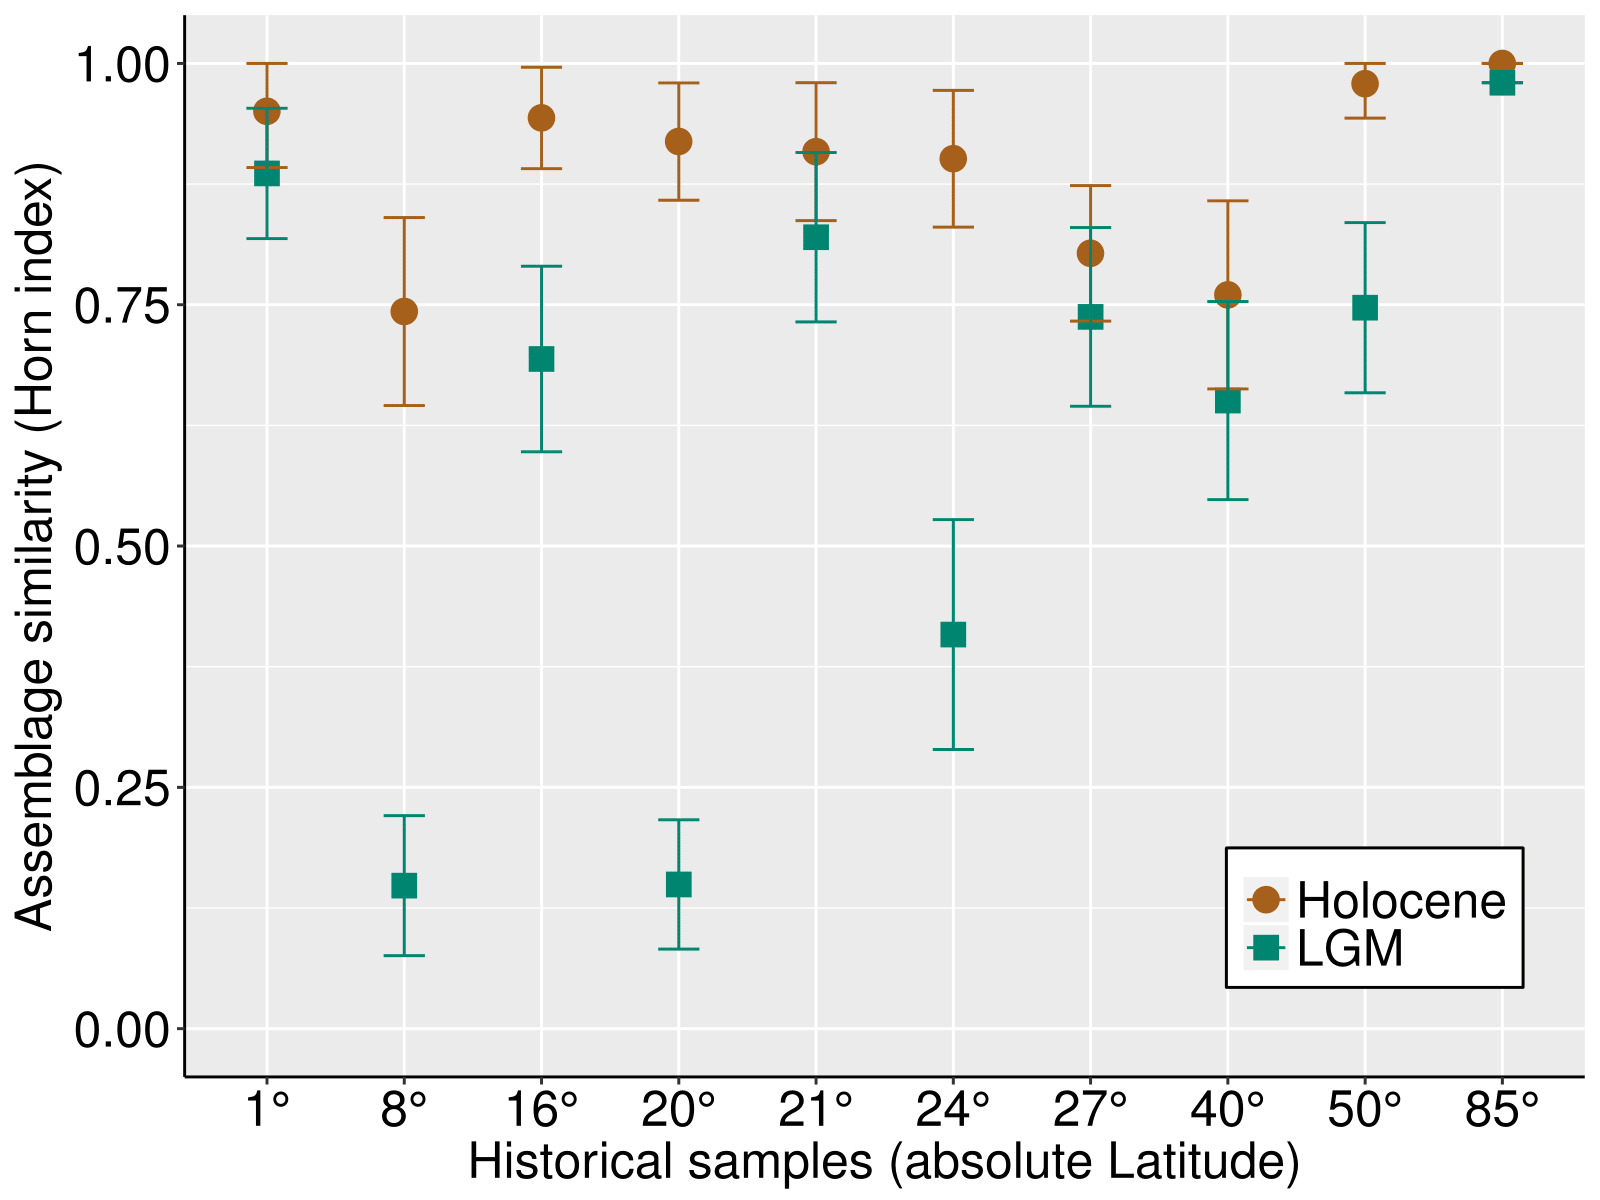
\includegraphics[scale=0.15]{fig_similarity.png}
		% \rule{35em}{0.5pt}
\end{figure}


% Bias: violin plot bias residuals & 95th percentile plot
\begin{figure}[htbp]
\caption{
Difference in shell size distributions between populations of the re-sampled assemblages and the Buckley Collection assemblages (in total, 65 populations of 20 species from ten samples). Species are coloured and ordered by shell size (larger sizes in purple-blue, smaller sizes in orange-yellow); species marked with ($*$) were present in the morphometric dataset.
\textbf{(a)} Residuals were calculated between the Buckley Collection and the re-sampled samples with respect to the identity function (1:1 relationship). Numbers indicate mean squared error (MSE), the 95th percentile metric shows the smallest MSE. 
\textbf{(b)} Plot of the 95th percentile of the population shell size distributions from the Buckley Collection against the re-sampled samples, line 1:1 represents the identity function. }
\label{fig_violin_95q}
\centering
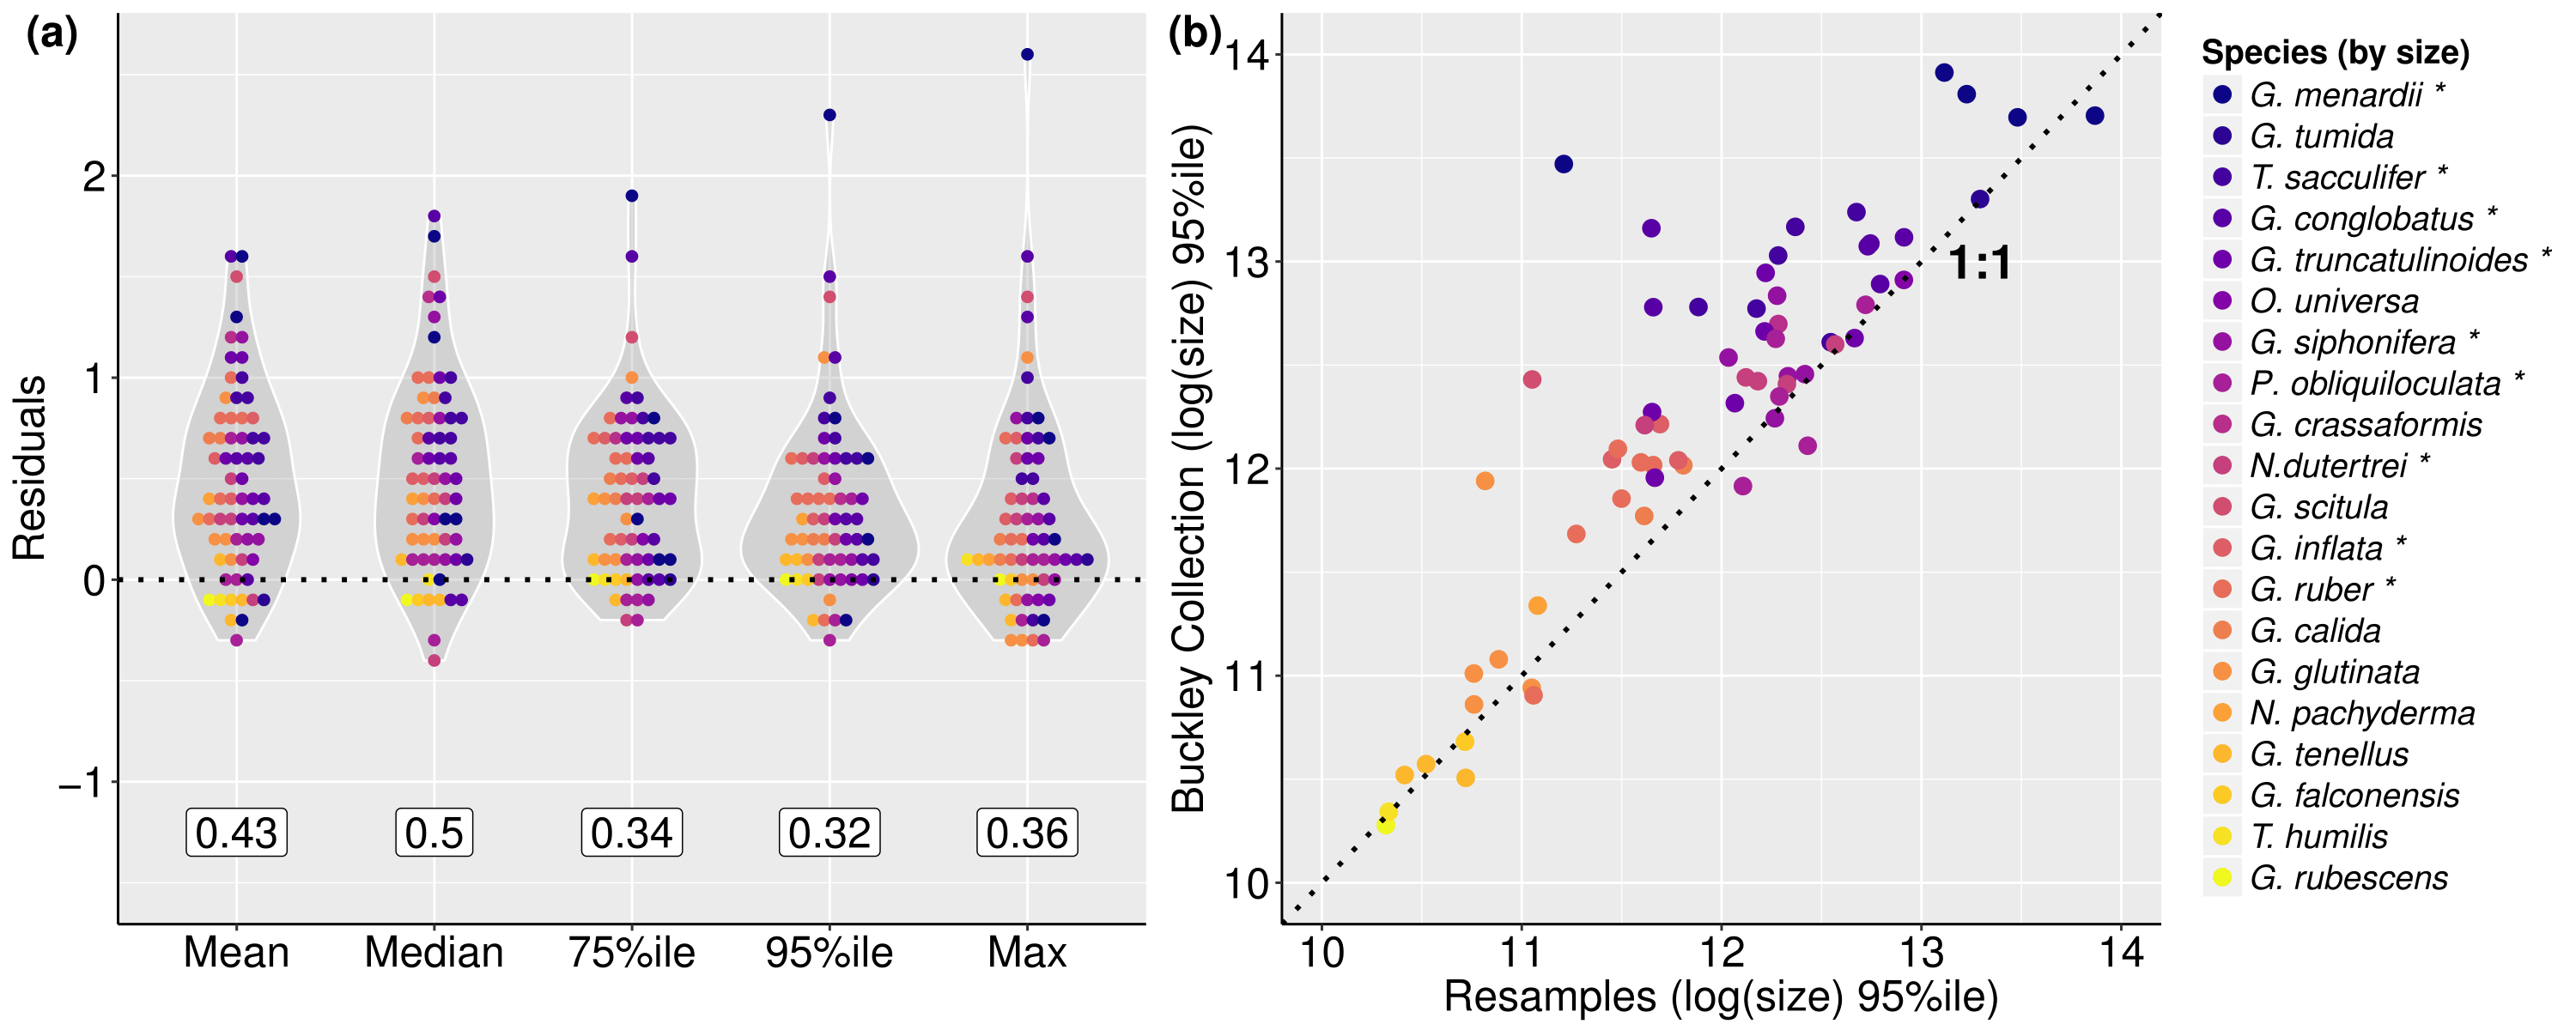
\includegraphics[scale=0.12]{fig_violin_95q.png}
		% \rule{35em}{0.5pt}
\end{figure}


\subsection{Shell size distributions}

The residuals of the regressions were predominantly positive (Fig. \ref{fig_violin_95q}a), and residuals increased with increasing species size \textcolor{red}{(Plot residuals as function of species size - Supp Info)}. This indicates that the Buckley Collection has a consistent collector bias towards large specimens. Henry Buckley personally carried out all the sample processing, isolation of foraminiferal specimens and their identification, thus the collector biases in his collection are likely to be systematic, especially for within-species comparisons. 
The mean squared error was lowest for the 95th percentile (Fig. \ref{fig_violin_95q}a), meaning that this metric is the least biased measurement of the Buckley Collection when considering log-transformed shell area.
\cite{schmidt2004size} also used the 95th percentile of the size distributions in PF assemblages because it is more robust to random sampling than the maximum size (which is easily distorted by a single outlier) and less sensitive to the sampling effort of picking smaller specimens than the distributions' mean and median values.


%----------------------------------------------------------------------------------------

\section{Discussion}

% Rarefaction curve MARGO
% Similarity among neighbouring samples MARGO
% bias of rare species

% If the lineages Buckley identified are a subsample of the lineages recognized by me, this indicates an incomplete representation of the assemblage, meaning that the sediment’s planktonic foraminiferal richness is not well represented in the Buckley collection. This type of taxonomic bias is critical for the use of the collection in analyses of planktonic foraminiferal communities and species coexistence, which will probably be a later section of my PhD. However, the current proposed project focuses on within lineage variation (intraspecific morphological variation, species’ abundance and genetic diversity), therefore this bias will not directly affect our analyses.



%----------------------------------------------------------------------------------------

\section{Conclusion}



%----------------------------------------------------------------------------------------

% OLD TEXT - check

% Taxonomic bias was assessed by comparing for each sample the species identified by us and the ones present in the Buckley Collection. Dissimilarity 

%  we expected that Buckley's species richness for each sample would be a subsample (i.e. nested) of the species richness found by us. A incomplete representation of the assemblage.

% If taxonomic bias is present there would be a mismatch between the lineages found in Buckley’s Collection and the ones found in my sample. If Buckley found lineages that were not observed by me, this might indicate he misidentified them. In this case, I will carefully re-analyse the high-resolution images of the potentially misidentified lineage in his collection to check whether that lineage was systematically misidentified. When the misidentification of a lineage is consistent throughout the collection, we will only use my samples’ specimens for the analysis. If, however, 
	
	
%Size bias can be detected as a bias towards larger specimens or larger lineages. The latter has the same effect as an incomplete representation of the assemblage, as it would mean that Buckley only identified a sub-sample (large lineages) of the full assemblage. Size bias towards larger individuals will be assessed by comparing the shell size distribution obtained from my re-sampling of the sediments and the one obtained from the Buckley collection. Shell size distributions were compared using statistical test. 

% If I find evidence of a specimen size bias in the collection, I will clarify for each lineage (i) how do the size distributions differ (in their average, their variance or in both)? (ii) Do the size distributions of a lineage differ in a systematic way (i.e. is the size bias consistent throughout the sediments where the lineage is found)? The answer to these questions will guide me on how to adjust my dataset to the biases found.

%Size distributions already have an artificial cut-off dictated by the mesh size of the sieve used when processing the bulk sediment. This artificial cut-off influences each lineage differently, because depending on the lineage’s average shell size the cut-off will eliminate a different portion of its population. % If the size bias in the Buckley collection is systematic among the populations within a lineage, we could parametrize it as an additional artificial cut-off. 

% I will determine the populational maximum shell size distribution based on Schmidt et al. (2004) methodology. They used the size value that separates the largest 5\% of shells (i.e. the 95th centile) and showed that this value is more correlated to the mean and median of the size distribution than the maximum value itself, because the maximum value is more dependent on random sampling (Schmidt et al. 2004). If the size bias is not systematic within lineages of the collection, then the adjustment of the collection morphometric dataset will depend on how the size distributions differ.  It might also be that not all populations of a lineage show size bias, allowing us to still use some populations for the analyses.


% If the size bias is not systematic within lineages of the collection, then the adjustment of the collection morphometric dataset will depend on how the size distributions differ.  It might also be that not all populations of a lineage show size bias, allowing us to still use some populations for the analyses.


%The original deposits, from which the Buckley collection was created, are still stored at the NHMUK Ocean-Bottom Deposits (OBD) Collection.  There is no record of how Buckley picked the specimens to amass his collection. However, since he personally carried out the sample processing, isolation of foraminiferal specimens and their identification, all biases in his collection are likely to be systematic, especially for within-species comparisons. The two main potential sources of bias are taxonomic bias (systematic misidentification or incomplete representation of the assemblage) and size bias (bias towards larger specimens or larger lineages).
% Because it is a systematic process, it will cause a distortion from the truth in a predictable (not random) direction.
% So, in the face of systematic error in an interval scale measurement, whether or not there is bias depends upon the measure of association in question.
% Is the difference due to a systematic error (bias) in the method - or simply to random error

%%% Sieve bias
%  Planktonic foraminifera are collected by washing the sediment through a sieve. The size of that sieve (e.g. 63 $\mu$m, 150 $\mu$m) will determine which individuals are retained and thus induce a size bias in the sample \citep{alsabouni2007vertical}. The sieve bias results in the truncation of the left tail of the size distribution. There is no record of which sieve-size Buckley used to picked the specimens to amass his collection. However, since he personally carried out the sample processing, isolation of foraminiferal specimens and their identification, the biases in his collection are likely to be systematic, especially for within-species comparisons. 
%  Size distributions already have an artificial cut-off dictated by the mesh size of the sieve used when processing the bulk sediment. This artificial cut-off influences each lineage differently, because depending on the lineage’s average shell size the cut-off will eliminate a different portion of its population. If the size bias in the Buckley collection is systematic among the populations within a lineage, we could parametrize it as an additional artificial cut-off. 

% Isabel Thesis
% Sieve size strongly affects within-sample species richness and rarefied richness, with larger mesh sizes unsurprisingly retaining fewer species. Generally finer sieve sizes produce more accurate estimates of diversity, as these contain both the larger and the smaller individuals (Al-Sabouni et al., 2007). Species that are relatively more abundant at small mesh sizes include G. falconensis, G. ruber, H. scitula, G. rubescens, N. incompta and T. quinqueloba, whereas G. conglobatus, T. sacculifer, H. hirsuta, M. menardii, T. truncatulinoides, G. tumida, O. universa and P. obliquiloculata become relatively less abundant. G. bulloides, G. siphonifera and G. inflata show opposite trends of diversity with mesh sites in different sites.

%----------------------------------------------------------------------------------------

\label{Bibliography}
\bibliographystyle{abbrvnat} % Use the agsm, abbrvnat, unsrtnat BibTeX style for formatting the Bibliography
\bibliography{bias-bibliography.bib} % The references (bibliography) information are stored in the file named "Bibliography.bib"



\end{document}  

